\chapter{関連技術}
本章では視覚刺激を用いて被験者の歩行速度を操作に関する研究を示し,本研究の位置づけを明らかにする.
\section{自己運動感覚に関する研究}
\subsection{身体運動と視覚刺激が自己運動感覚に及ぼす影響}
近藤らは被験者の移動時に\figref{fig:1}のようなベクションを用いた視覚刺激が自己運動感覚へと与える影響を調べた\cite{kondo}.
その結果,移動環境や移動方法により視覚刺激による自己運動感覚に与える影響が変化することは確認されなかった.
しかし,それぞれの実験項目で主観速度が速くなったことは確認された.
\begin{figure}[h]
    \centering
    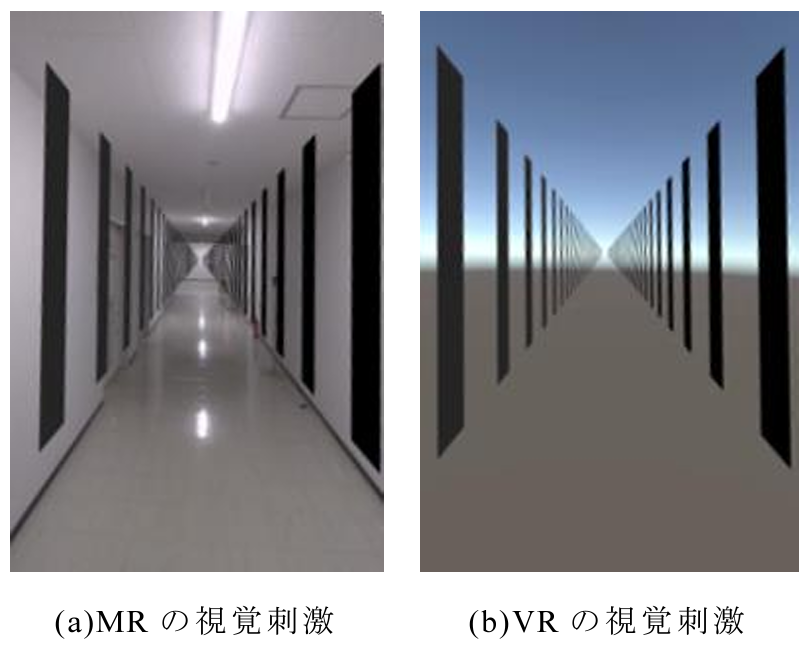
\includegraphics[clip, width=0.8\linewidth]{fig/1.PNG}
    \caption{近藤らの実験で使用された視覚刺激}
    \label{fig:1}
\end{figure}

\subsection{歩行における視覚と運動感覚の整合性}
高幣らは歩行する際に感じる足の接地や筋肉の伸縮などを歩行運動感覚と定義し,
HMDで被験者に対して\figref{fig:2}のような一定速度で空間内を前進する映像を提示し,この提示した速度を視覚速度を定義した.
これらの歩行運動感覚と視覚速度を入出力とし,
自己移動速度のそれぞれの感覚における速度知覚特性とその関係について調べた\cite{takahei}.
その結果,視覚で知覚される移動速度は常に歩行運動感覚で知覚される速度よりも遅く知覚されることがわかった.
\begin{figure}[h]
    \centering
    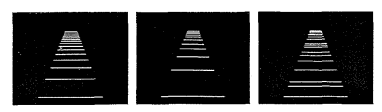
\includegraphics[clip, width=0.9\linewidth]{fig/2.PNG}
    \caption{高幣らの実験でHMDに提示される映像}
    \label{fig:2}
\end{figure}


\section{歩行誘導に関する事例}
路面や標識に印字された記号や文字,警備員による音声案内などの意味を解釈して行動に移させる情報提示を用いず,
意味解釈を必要とせずに歩行者を誘導可能な手法について数多く研究されている.
これらの手法では提示の意味について解釈する過程を必要とせず,
対象者のリソースを消費しないナビゲーション手法として注目されている.
これまでに提案されている手法には,視覚以外の刺激を利用したものと,
本研究と同様に視覚を利用したものがある.

\subsection{視覚以外を使用した歩行誘導方法}
Kojimaらは耳が引っ張ることで歩行ナビゲーションを行う手法であるPull-Naviを提案した\cite{kojima}.
Pull-Naviの概要を\figref{fig:6}に示す.
実験した結果,右左の耳を右左に引っ張ると,被験者はどうしても右,に動きたくなることを確認した.
また,両耳を前方に引っ張ると速く,後方に引っ張ると被験者は遅く歩きたくなったという結果を確認した.
しかし,この手法では耳を引っ張ることで身体に触覚刺激を与えているため,被験者を不快に感じさせる可能性がある.
\begin{figure}[H]
    \centering
    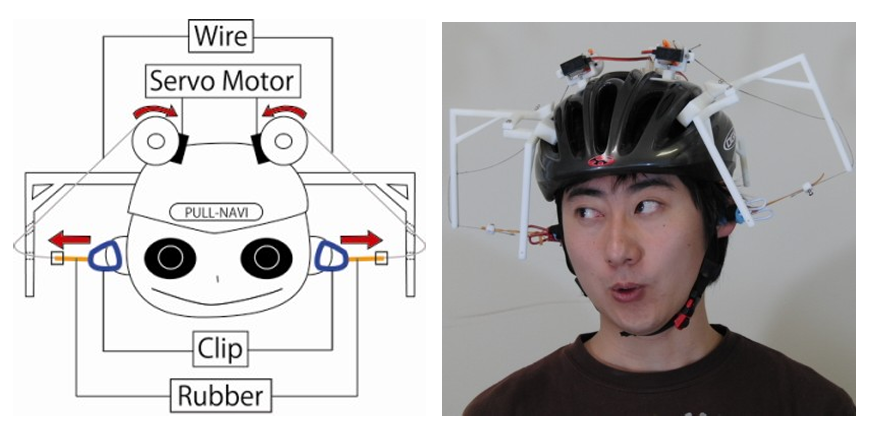
\includegraphics[clip, width=0.8\linewidth]{fig/6.PNG}
    \caption{Pull-Naviの概要図}
    \label{fig:6}
\end{figure}



Freyらは靴の底を傾けて体勢を変化させることで歩行誘導を行う手法を提案した\cite{Frey}.
このシステムでは,靴底に仮想の拡張地形(\figref{fig:10})に変換された道を歩くことになる.
しかし,この手法では靴が傾くことによって足元が不安定になるため,転倒の危険性がある.
\begin{figure}[H]
    \centering
    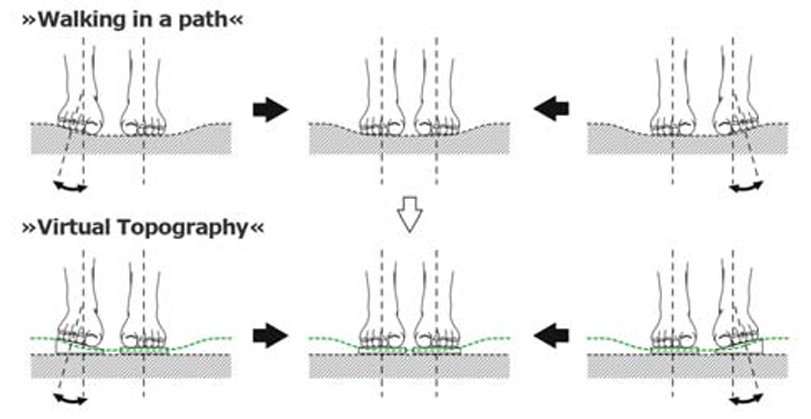
\includegraphics[clip, width=0.8\linewidth]{fig/10.PNG}
    \caption{拡張地形について}
    \label{fig:10}
\end{figure}


\section{視覚刺激を用いた歩行速度制御}
人は五感によって得られる情報のうち,視覚によるものは87\%を占めており,人の行動に大きな影響を及ぼすことが知られている\cite{syomei}.
このことから,視覚刺激は歩行速度制御に適しており,以下のような研究が行われている.
\subsection{プロジェクションマッピングを用いた歩行速度制御}
上田らはプロジェクションマッピングを用いて床にベクション効果を伴う映像\figref{fig:4}を投影し,
被験者に対し,身体的な負担をかけず,無意識に歩行速度を制御できるかを調べた\cite{ueda}.実験環境を\figref{fig:3}に示す.
その結果,プロジェクションマッピングを用いたベクション効果を伴う映像は歩行速度に変化をもたらすことがわかった.
しかし,課題として暗所を歩行する際の安全性の低さが挙げられた.
\begin{figure}[H]
    \centering
    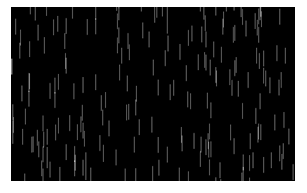
\includegraphics[clip, width=0.6\linewidth]{fig/4.PNG}
    \caption{ベクション効果を伴う映像}
    \label{fig:4}
\end{figure}
\begin{figure}[H]
    \centering
    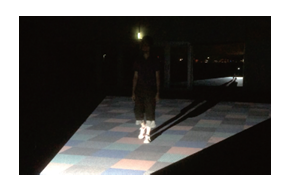
\includegraphics[clip, width=0.6\linewidth]{fig/3.PNG}
    \caption{プロジェクションマッピングにより足元に映像を提示されている被験者}
    \label{fig:3}
\end{figure}





\subsection{周辺視野への刺激提示による速度感増強}
岡野らは周辺視野に対して適切なオプティカルフロー(OF)を提示することによって,
自己運動感覚の中の速度感覚を増強できるかを調べた\cite{okano}.
実験で使用した周辺視ディスプレイを\figref{fig:oka}に示す.
結果として,歩行時の速度感覚が増強されるという効果はあると確認された.
しかし,視野下部に対する刺激と視野側面に対する刺激に関する問題が残っている.
\begin{figure}[H]
    \centering
    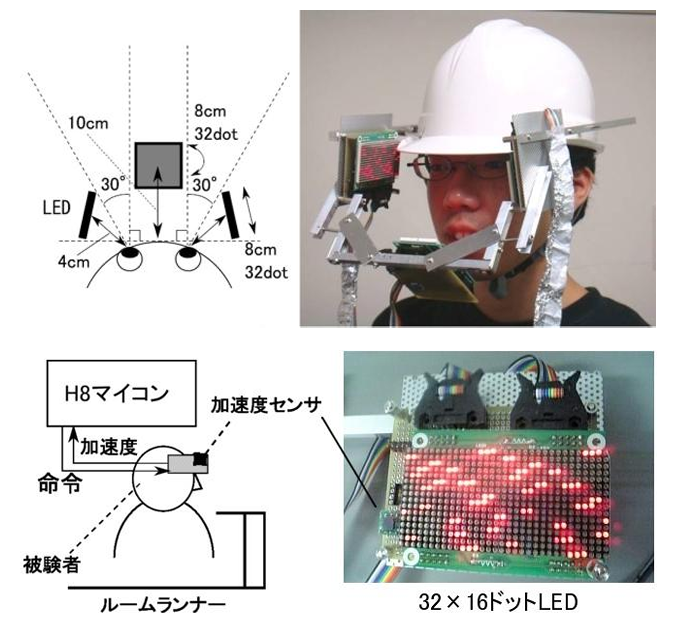
\includegraphics[clip, width=0.7\linewidth]{fig/9.PNG}
    \caption{周辺視野にオプティカルフローを提示するシステム}
    \label{fig:oka}
\end{figure}



\subsection{視覚刺激と身体動揺を利用した歩行誘導}
オプティカルフローは自分の移動の方向と速度を判断する重要な手掛かりとなっている\cite{opu}.
Anoukらはオプティカルフローの速度の変化に応じて被験者が歩行速度を調節できるかをVR空間を使用して調べた\cite{Anouk}.
\figref{fig:9}に実験で用いたVR空間を示す.
結果として知覚するOFの速度が遅いと歩行速度は速く,
逆にOFの速度が速いと歩行速度は遅くなる傾向にあると分かった.
\begin{figure}[H]
    \centering
    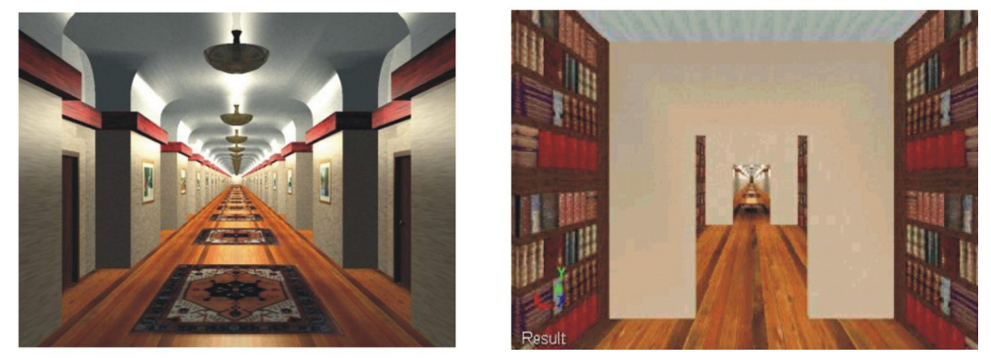
\includegraphics[clip, width=0.9\linewidth]{fig/12.PNG}
    \caption{オプティカルフローを提示するVRシステム}
    \label{fig:9}
\end{figure}


\section{VRを用いた歩行速度制御}
谷崎らは実空間を歩行中の被験者にヘッドマウントディスプレイを通してオプティカルフローの速度と中心視野を変化させたバーチャル空間\figref{fig:5}を提示し,
被験者の歩行速度の変化を調べた\cite{tanizaki}.
その結果,オプティカルフローの速度と被験者の歩行速度の間に負の相関があると示唆された.

\begin{figure}[H]
    \centering
    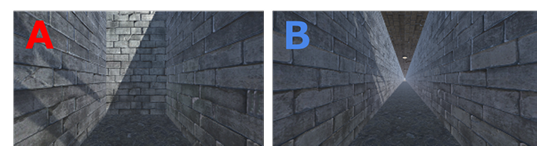
\includegraphics[clip, width=1.0\linewidth]{fig/5.PNG}
    \caption{実験で使用されたバーチャル空間}
    \label{fig:5}
\end{figure}

谷崎らは.VR空間内で並走するバーチャルアバタの並進の
速度,形態,歩行運動の動きの3つの要因に対して自然歩行時の歩行速度が
変化するかを調べた\cite{heiso}.
並走するバーチャルアバタの存在するバーチャル空間を\figref{fig:15}に示す.
その結果,並走するアバタの形態と運動による歩行速度変調が確認された.
しかし,長距離や長時間,実験環境外の環境でのシステムの有用性は確認できていない.
\begin{figure}[H]
    \centering
    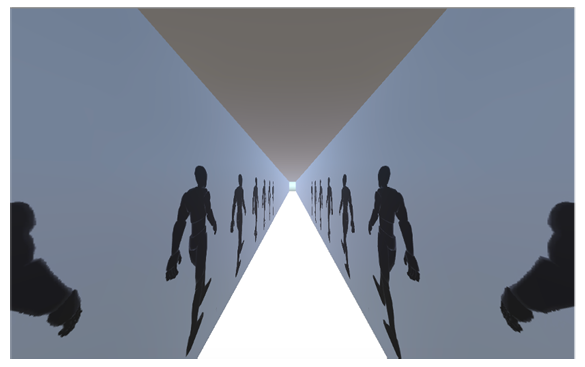
\includegraphics[clip, width=0.9\linewidth]{fig/15.PNG}
    \caption{実験で使用された並走するバーチャルアバタの存在するバーチャル空間}
    \label{fig:15}
\end{figure}


これらの手法はVRに基づいており,現実空間の歩行速度誘導に利用するのことは難しい.

\section{ARを用いた歩行速度制御}
櫻木らはARグラスを通して見える床面上に「動く歩道」のテクスチャをアニメーション提示し,
その際の被験者の歩行運動を観察した\cite{sakura}.
この手法はARに基づいており,現実空間の歩行速度誘導への適合性が高いものの,
著者らが期待した誘導効果は確認できなかった.
その理由として,ARで提示したテクスチャの見た目(\figref{fig:8})が現実の床面の見た目と差があること,
歩行の際にテクスチャの隙間から床面が見えてしまい,被験者からみた現実感(被験者から見える空間の整合性)が低下したことの影響を挙げている.

\begin{figure}[H]
    \centering
    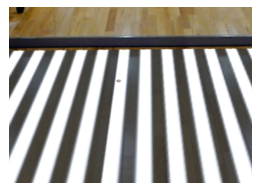
\includegraphics[clip, width=0.9\linewidth]{fig/8.PNG}
    \caption{実験で使用されたテクスチャ}
    \label{fig:8}
\end{figure}
\section{本稿の位置付け}
本研究では個々の歩行者に対し,確実な指示伝達を行うのにARが適していると考える.
また,ARを用いた行動制御方法では実際の歩行面に近いテクスチャーをトラベレーターのようにアニメーションすることで
拡張現実的なアプローチでも誘導効果が得られ,被験者の動きをより制御できると考える\cite{moto}.
本稿では芝生道にて,芝生を模したバーチャル床を表示した場合と芝生を模していないバーチャル床を表示した場合
を比べて被験者の歩行速度制御に有位性が出るか否かの調査する.